\documentclass[12pt,a4paper]{../krautsourcing/homework}
\usepackage[utf8]{inputenc}
\usepackage[ngerman]{babel}
\usepackage[T1]{fontenc}
\usepackage{amsmath}
\usepackage{graphicx}
\usepackage{amsfonts}
\usepackage{amssymb}
\usepackage{lmodern}
\usepackage{amsmath}
\usepackage{amssymb}
\usepackage{paralist}
\usepackage{tabularx}
\usepackage{tikz}
\usepackage{mathtools}
\usetikzlibrary{automata,petri,positioning,calc}

\author{Ruben Felgenhauer,\\Alexander Hildebrandt,\\Leonhard Reichenbach}
\datef{29}{11}{2015}
%\date{\today}
\course{Formale Grundlagen der Informatik II}
\sheet{7}
\sectionprefix{Übungsaufgabe \thesheet.}
\subsectionprefix{\thesheet.}
\subsubsectioncounter{\alph{subsubsection}}
\group{06}
\subsubsectionprefix{(}
\subsubsectionsuffix{)}

\newcommand{\tc}[1]{\footnotesize{\(#1\)}}
\newcommand{\m}[1][]{\textbf{m}_{\textbf{#1}}}
\newcommand{\cvec}[1]{\begin{pmatrix}#1\end{pmatrix}}
\newcommand{\td}{0.75mm}

\begin{document}

\makeheadline

\addtocounter{section}{2}

\section{}

\subsection{}

\centerline{
\begin{tikzpicture}[auto,baseline,node distance=20mm]
\node[initial,initial text={}] (110) {\(p_1, p_2\)};
\node[right=of 110]            (020) {\(p_2(2)\)};
\node[right=of 020]            (001) {\(p_3\)};
\node[right=of 001]            (010) {\(p_2\)};
\node[below=of 110]            (200) {\(p_1(2)\)};
\node[at=(010|-200)]           (100) {\(p_1\)};
%
\path[->,shorten <=1mm, shorten >=1mm]
	($(110.east)+(0,\td)$)   edge node[above] {\tc{t_1}} ($(020.west)+((0,\td)$)
	($(110.south)+(-\td,0)$) edge node[left]  {\tc{t_2}} ($(200.north)+(-\td,0)$)
	($(020.west)+(0,-\td)$)  edge node[below] {\tc{t_2}} ($(110.east)+((0,-\td)$)
	(020.east)               edge node[above] {\tc{t_4}} (001.west)
	(001.east)               edge node[above] {\tc{t_3}} (010.west)
	($(010.south)+(-\td,0)$) edge node[left]  {\tc{t_2}} ($(100.north)+(-\td,0)$)
	($(200.north)+(\td,0)$)  edge node[right] {\tc{t_1}} ($(110.south)+((\td,0)$)
	($(100.north)+(\td,0)$)  edge node[right] {\tc{t_1}} ($(010.south)+((\td,0)$)
; %-path-%
\end{tikzpicture}
}

\subsection{}

\begin{align*}
	\sigma \coloneqq p_1,p_2 \xrightarrow{t_2} p_1(2) \xrightarrow{t_1} p_1,p_2 \xrightarrow{t_1} p_2(2) \xrightarrow{t_4} p_3 \xrightarrow{t_3} p_2 \xrightarrow{t_2} p_1
\end{align*}

\subsection{}

\begin{compactenum}
\item 
Nach der Schaltfolge \(\sigma\) hat das Netz die Markierung \(\m = p_1\).
Hier können wir nur \(t_1\) schalten, und erhalten die Markierung \(p_2\). Von hier aus können wir nur \(t_2\) schalten und gelangen zurück zu \(p_1\). Somit können wir von jedem von \(\m\) aus erreichbaren Zustand also eine Transition schalten und das Netz ist in \(\m\) verklemmungsfrei.
\item
Das Netz ist nicht lebendig, da wir in \(p_1\) und \(p_2\) weder \(t_3\) noch \(t_4\) schalten können.
\end{compactenum}

\subsection{}

\begin{align*}
	\sigma = \cvec{1\\1\\0\\0} 
	\xrightarrow{t_2} \cvec{2\\0\\0\\0}
	\xrightarrow{t_1} \cvec{1\\1\\0\\0}
	\xrightarrow{t_1} \cvec{0\\2\\0\\0}
	\xrightarrow{t_4} \cvec{0\\0\\1\\0}
	\xrightarrow{t_3} \cvec{0\\1\\0\\0}
	\xrightarrow{t_2} \cvec{1\\0\\0\\0}
\end{align*}

\newpage

\subsection{}

Zum gegebenen Petrinetz \ \(\mathcal{N} = (P,T,F,W,\m[0])\) konstruieren wir ein Petrinetz \ \(\mathcal{N}' = (P,T,F,W',\m[0])\) mit \(W': (p,t) \mapsto 1\).\\
In unserem Fall ändert sich also nur, dass nun \(W(p_2,t_4) = 1\) gilt:\\
\centerline{
\begin{tikzpicture}[auto,baseline,node distance=20mm,transition/.style={draw,minimum width=1cm}]
	\node[place,tokens=1,label=above left:\(p_1\)]                    (p1) {};
	\node[place,tokens=1,below right=of p1,label=above right:\(p_2\)] (p2) {};
	\node[place,below right=of p2,label=below right:\(p_3\)]          (p3) {};
	\node[transition,at=(p2|-p1)] (t1) {\(t_1\)};
	\node[transition,at=(p1|-p2)] (t2) {\(t_2\)};
	\node[transition,at=(p3|-p2)] (t3) {\(t_3\)};
	\node[transition,at=(p2|-p3)] (t4) {\(t_4\)};
	\path[->]
		(p1) edge (t1) (t1) edge (p2)
		(p2) edge (t2) (t2) edge (p1)
		(p3) edge (t3) (t3) edge (p2)
		(p2) edge (t4) (t4) edge (p3)
	; %-path-%
\end{tikzpicture}
}
Dadurch verändert sich der Erreichbarkeitsgraph folgendermaßen:\\
\centerline{
\begin{tikzpicture}[auto,baseline,node distance=20mm]
\node[initial,initial text={},initial where=above] (110) {\(p_1,p_2\)};
\node[left=of 110]                                 (200) {\(p_1(2)\)};
\node[right=of 110]                                (020) {\(p_2(2)\)};
\node[right=of 020]                                (011) {\(p_2,p_3\)};
\node[right=of 011]                                (002) {\(p_3(2)\)};
\node[below=of 020]                                (101) {\(p_1,p_3\)};
%
\path[->,shorten <=1mm, shorten >=1mm]
	($(110.east)+(0,\td)$)   edge                node[above]       {\tc{t_1}} ($(020.west)+(0,\td)$)
	($(110.west)+(0,-\td)$)  edge                node[below]       {\tc{t_2}} ($(200.east)+(0,-\td)$)
	($(110.south)+(\td,0)$)  edge[bend right=45] node[above right] {\tc{t_3}} ($(101.west)+(0,\td)$)
	($(200.east)+(0,\td)$)   edge                node[above]       {\tc{t_1}} ($(110.west)+(0,\td)$)
	($(020.west)+(0,-\td)$)  edge                node[below]       {\tc{t_2}} ($(110.east)+(0,-\td)$)
	($(020.east)+(0,\td)$)   edge                node[above]       {\tc{t_4}} ($(011.west)+(0,\td)$)
	($(011.west)+(0,-\td)$)  edge                node[below]       {\tc{t_3}} ($(020.east)+(0,-\td)$)
	($(011.east)+(0,\td)$)   edge                node[above]       {\tc{t_4}} ($(002.west)+(0,\td)$)
	($(011.south)+(-\td,0)$) edge[bend left=45]  node[above left]  {\tc{t_2}} ($(101.east)+(0,\td)$)
	($(002.west)+(0,-\td)$)  edge                node[below]       {\tc{t_3}} ($(011.east)+(0,-\td)$)
	($(101.west)+(0,-\td)$)  edge[bend left=45]  node[below left]  {\tc{t_4}} ($(110.south)+(-\td,0)$)
	($(101.east)+(0,-\td)$)  edge[bend right=45] node[below right] {\tc{t_1}} ($(011.south)+(\td,0)$)
; %-path-%
\end{tikzpicture}\\
}
\begin{compactenum}
\item
Wie man am Erreichbarkeitsgraphen sieht, existieren zu jedem Übergang \(\m[1] \xrightarrow{t_{12}} \m[2]\) ein entgegengerichteter Übergang \(\m[2] \xrightarrow{t_{21}} \m[1]\). Durch diese Eigenschaft existiert zu jeder Markierung \(\m\) eine Schaltfolge \(\sigma\), sodass \(\m \xrightarrow{\sigma} \m[0]\) gilt. Somit ist \(\mathcal{N}'\) reversibel.
\item
Wie in 7.3.3 ist \(\mathcal{N}'\) verklemmungsfrei, da wir zu jeder Markierung \(\m\) eine aktivierte Transition finden können.
\item
Außerdem ist \(\mathcal{N}'\) beschränkt, da der Erreichbarkeitsgraph beschränkt ist.
\end{compactenum}
Die Lösung funktioniert immer dann, wenn alle Stellen im Netz einen Pfad zu jeder anderen Stelle besitzen, und es keine Transition gibt, die die Gesamtzahl der Marken im Netz verringert.

\subsection{}

Das eben konstruierte Netz \(\mathcal{N}'\) ist bereits lebendig, da wir im Erreichbarkeitsgraphen sehen können, dass für jede Markierung \(\m \in R(\mathcal{N}')\) und jede Transition \(t \in T(\mathcal{N}'')\) eine Schaltfolge \(\sigma\) existiert, sodass \(\m \xrightarrow{\sigma t} \m'\) gilt.\\
Der Erreichbarkeitsgraph ist 7.3.5 zu entnehmen.\\
Zudem ist das Netz ebenfalls:\\
\begin{compactenum}
\item reversibel (siehe 7.3.5)
\item verklemmungsfrei (siehe 7.3.5)
\item beschränkt (siehe 7.3.5)
\end{compactenum}

\stepcounter{section}

\section{}

\stepcounter{subsection}

\subsection{}

Das erste Kanal-Instanz-Netz lautet:\\
\centerline{
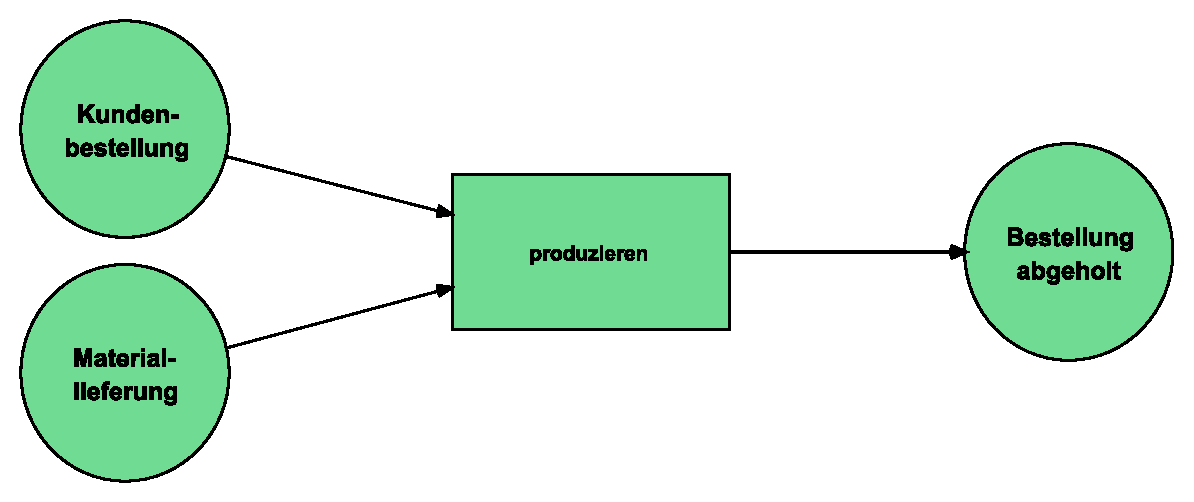
\includegraphics[scale=0.5,trim={0mm 0mm 0mm 0mm},clip]{Aufgabe_7-5/Aufgabe_7-5-1-1.pdf}
}\\
Über die Epifaltung \(\phi_1\) verfeinern wir das Netz:\\
\(
\begin{aligned}
\phi_1:
&\{(\textit{Kundenbestellung}), (\textit{Aus dem Briefkasten nehmen}), (\textit{Bestellungsordner})\}\\
&\mapsto \{(\textit{Kundenbestellung})\}\\
&\{(\textit{Matieriallieferung}), (\textit{Gegen Gutschrift an Firma liefern}), (\textit{Lager})\} \\
&\mapsto \{(\textit{Materiallieferung})\}\\
&\{(\textit{Bestellung auslesen}), (\textit{Material verarbeiten}), (\textit{Fertiges Produkt}), (\textit{Ware ins Schließfach legen})\} \\
&\mapsto \{(\textit{produzieren})\}\\
&\{(\textit{Zur Abholung bereit}), (\textit{Gegen Gutschrift entnehmen}), (\textit{Bestellung abgeholt})\} \\
&\mapsto \{(\textit{Bestellung abgeholt})\}
\end{aligned}
\)
\centerline{
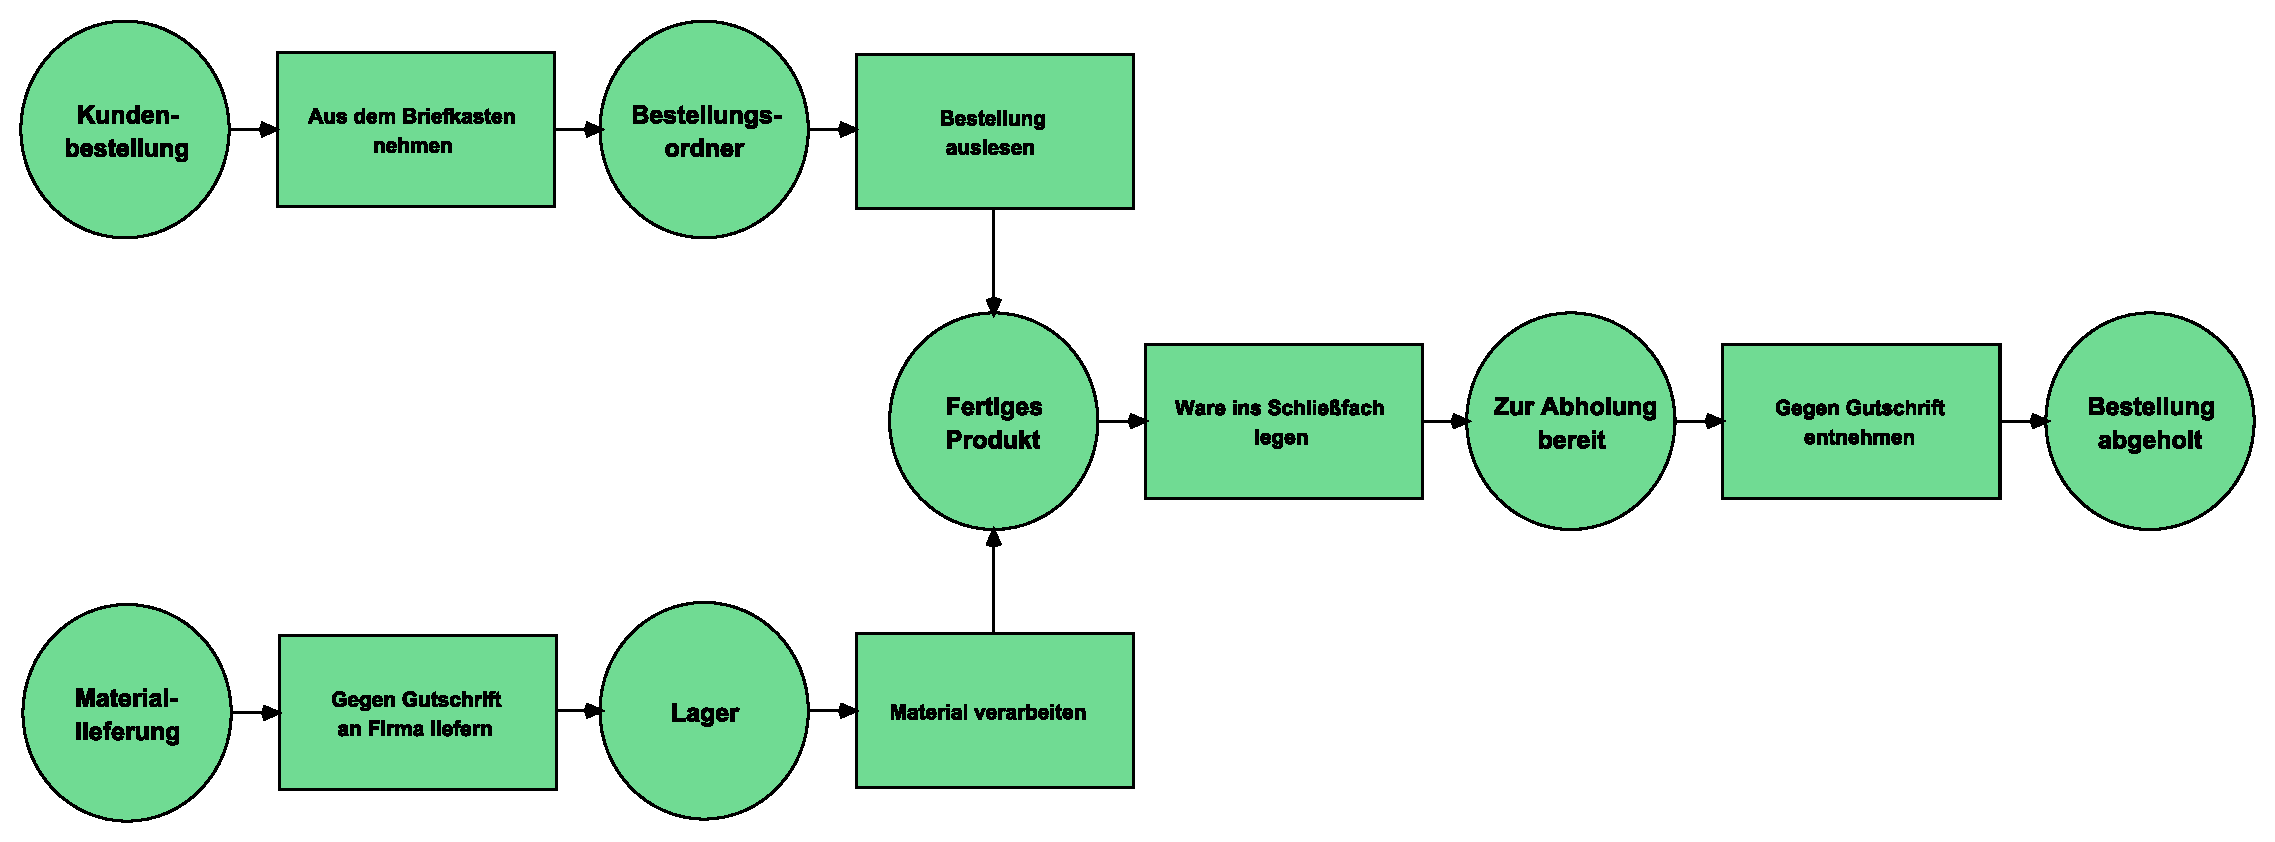
\includegraphics[scale=0.45,trim={0mm 0mm 0mm 0mm},clip]{Aufgabe_7-5/Aufgabe_7-5-1-2.pdf}
}
Das Netz wird erneut verfeinert über die Faltung \(\phi_2\):\\
\(
\begin{aligned}
\phi_2:& \{(\textit{Kundenbestellung}), (\textit{Aus dem Briefkasten nehmen}), (\textit{Bestellungsordner})\}\\
&\mapsto \{(\textit{Kundenbestellung})\}\\
&\{(\textit{Matieriallieferung}), (\textit{Firmenkonto}), (\textit{Gegen Gutschrift an Firma liefern}), (\textit{Lager})\} \\
&\mapsto \{(\textit{Materiallieferung})\}\\
&\{(\textit{Bestellung auslesen}), (\textit{Material verarbeiten}), (\textit{Fertiges Produkt}), (\textit{Qualitätskontrolle}),\\
&(\textit{Zufriedenstellendes Produkt}), (\textit{Ware ins Schließfach legen})\} \\
&\mapsto \{(\textit{produzieren})\}\\
&\{(\textit{Zur Abholung bereit}), (\textit{Gegen Gutschrift entnehmen}), (\textit{Bestellung abgeholt})\}\\
&\mapsto \{(\textit{Bestellung abgeholt})\}
\end{aligned}
\)\\
\centerline{
\includegraphics[scale=0.35,trim={0mm 0mm 0mm 0mm},clip]{Aufgabe_7-5/Aufgabe_7-5-1-3.pdf}
}

\subsection{}

\centerline{
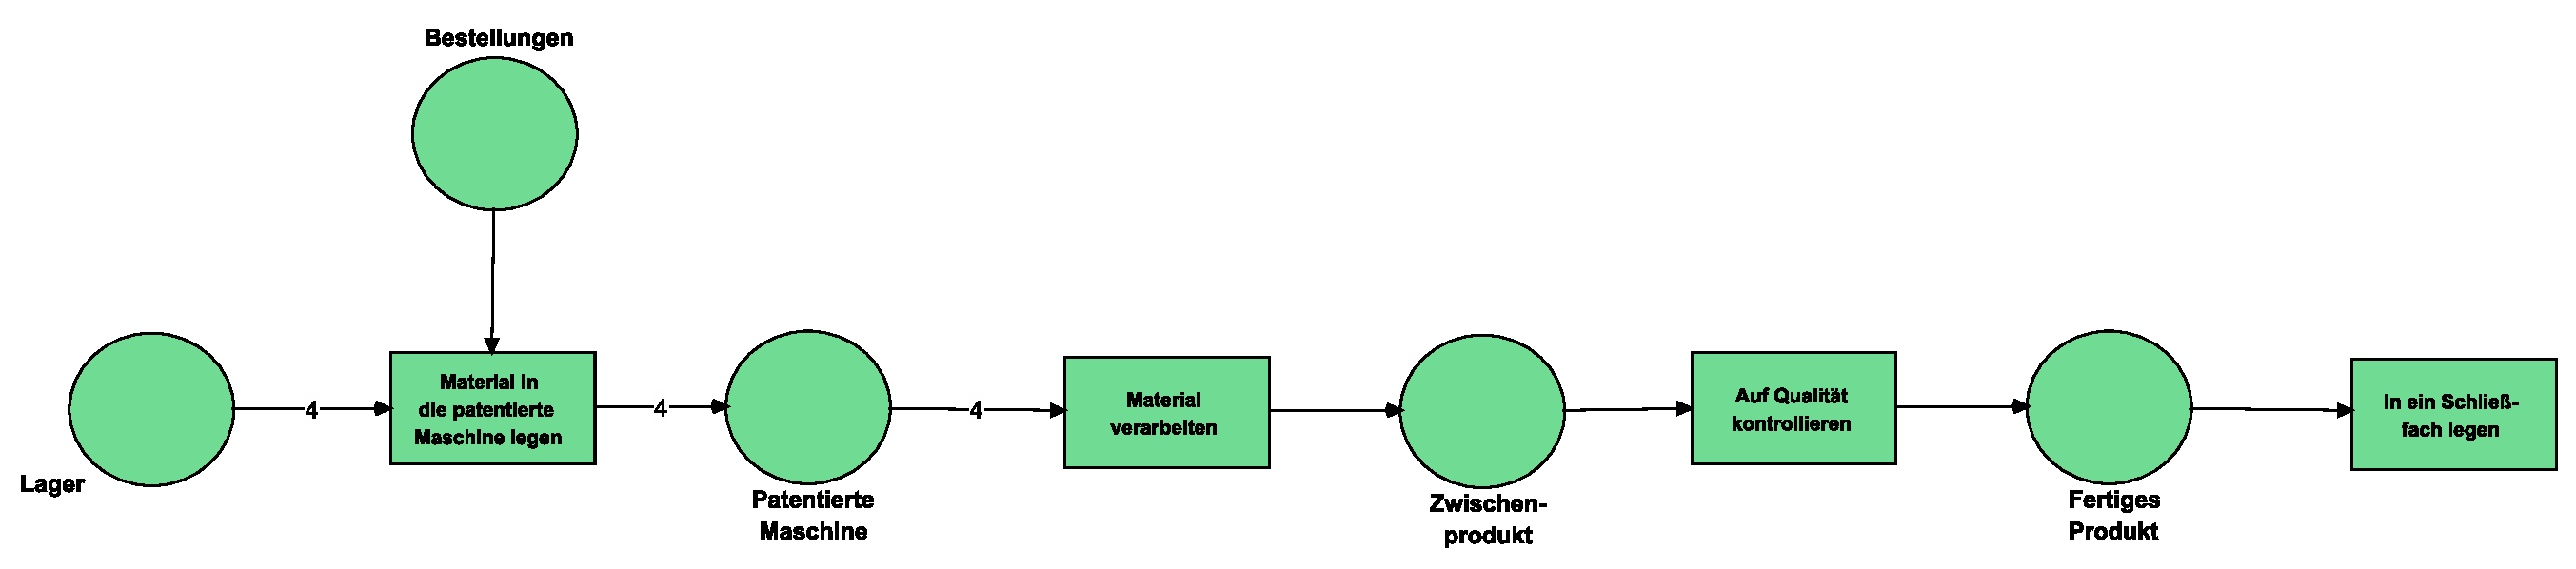
\includegraphics[scale=0.35,trim={0mm 0mm 0mm 0mm},clip]{Aufgabe_7-5/Aufgabe_7-5-3.pdf}
}

\subsection{}

\centerline{
\includegraphics[scale=0.3,trim={0mm 0mm 0mm 0mm},clip]{Aufgabe_7-5/Aufgabe_7-5-4.pdf}
}

\subsection{}
\begin{compactenum}[\bfseries a)]
\item
\textbf{Nebenläufigkeit:} Ist gegeben, da nebenläufig produziert und neue Bestellung entgegen genommen werden können
\item
\textbf{Lebendigkeit:} Ist gegeben, da wir in zwei Transitionen Marken erstellen, die durch alle Transitionen laufen, bis sie abgebaut werden.
\item
\textbf{Determinismus:} Durch die Nebenläufigkeit im Netz ist ein Nichtdeterminismus gegeben, da wir nicht absehen können, welche Transition als nächstes schaltet.
\item
\textbf{Beschränktheit:} Ist nicht gegeben, da wir zwei Transitionen haben, die unendlich oft Marken produzieren können, ohne das Marken aufgebraucht werden müssen.
\item
\textbf{Rücksetzbarkeit:} Ist gegeben, da man bei jeder möglichen Markierung einfach durch Schalten der vorliegenden Stellenkette die Markierung bei \glqq Abholung gegen Gutschrift\grqq \ abbauen kann.
\end{compactenum}

\subsection{}

\begin{compactitem}
\item
Gutschriften werden nicht aus den Schließfächern genommen
\item
Gutschriften sind nicht durch einen Betrag definiert; Falls man ein Firmenkonto einbauen will, das Gutschriften der Besteller annimmt und Gutschriften an die Lieferanten verteilt, hat man keine Kantengewichte vorgegeben und Markierungen können dadurch verschwinden.
\item
Es ist unklar was mit Produkten passiert, die durch die Qualitätskontrolle fallen.
\item
Briefkästen, Lager und Schließfächer sind unendlich groß
\end{compactitem}
Falls man die Vorgänge protokollieren möchte, muss man theoretisch an jede Transition eine neue Stelle hängen, die als Protokoll jeweiligen Transition dient, weil in jedem Schritt ein Fehler passieren kann. Wenn man nur ein Protokoll am Anfang setzt, ist es unklar, ob überhaupt produziert wurde. Falls erst am Ende ein Protokoll genommen wird, würden Fehler in der Produktion ignoriert statt protokolliert. Da diese Protokollierung trivial ist, wird sie im folgenden P/T-Netz nicht umgesetzt, um die Übersichtlichkeit zu fördern.\\
\centerline{
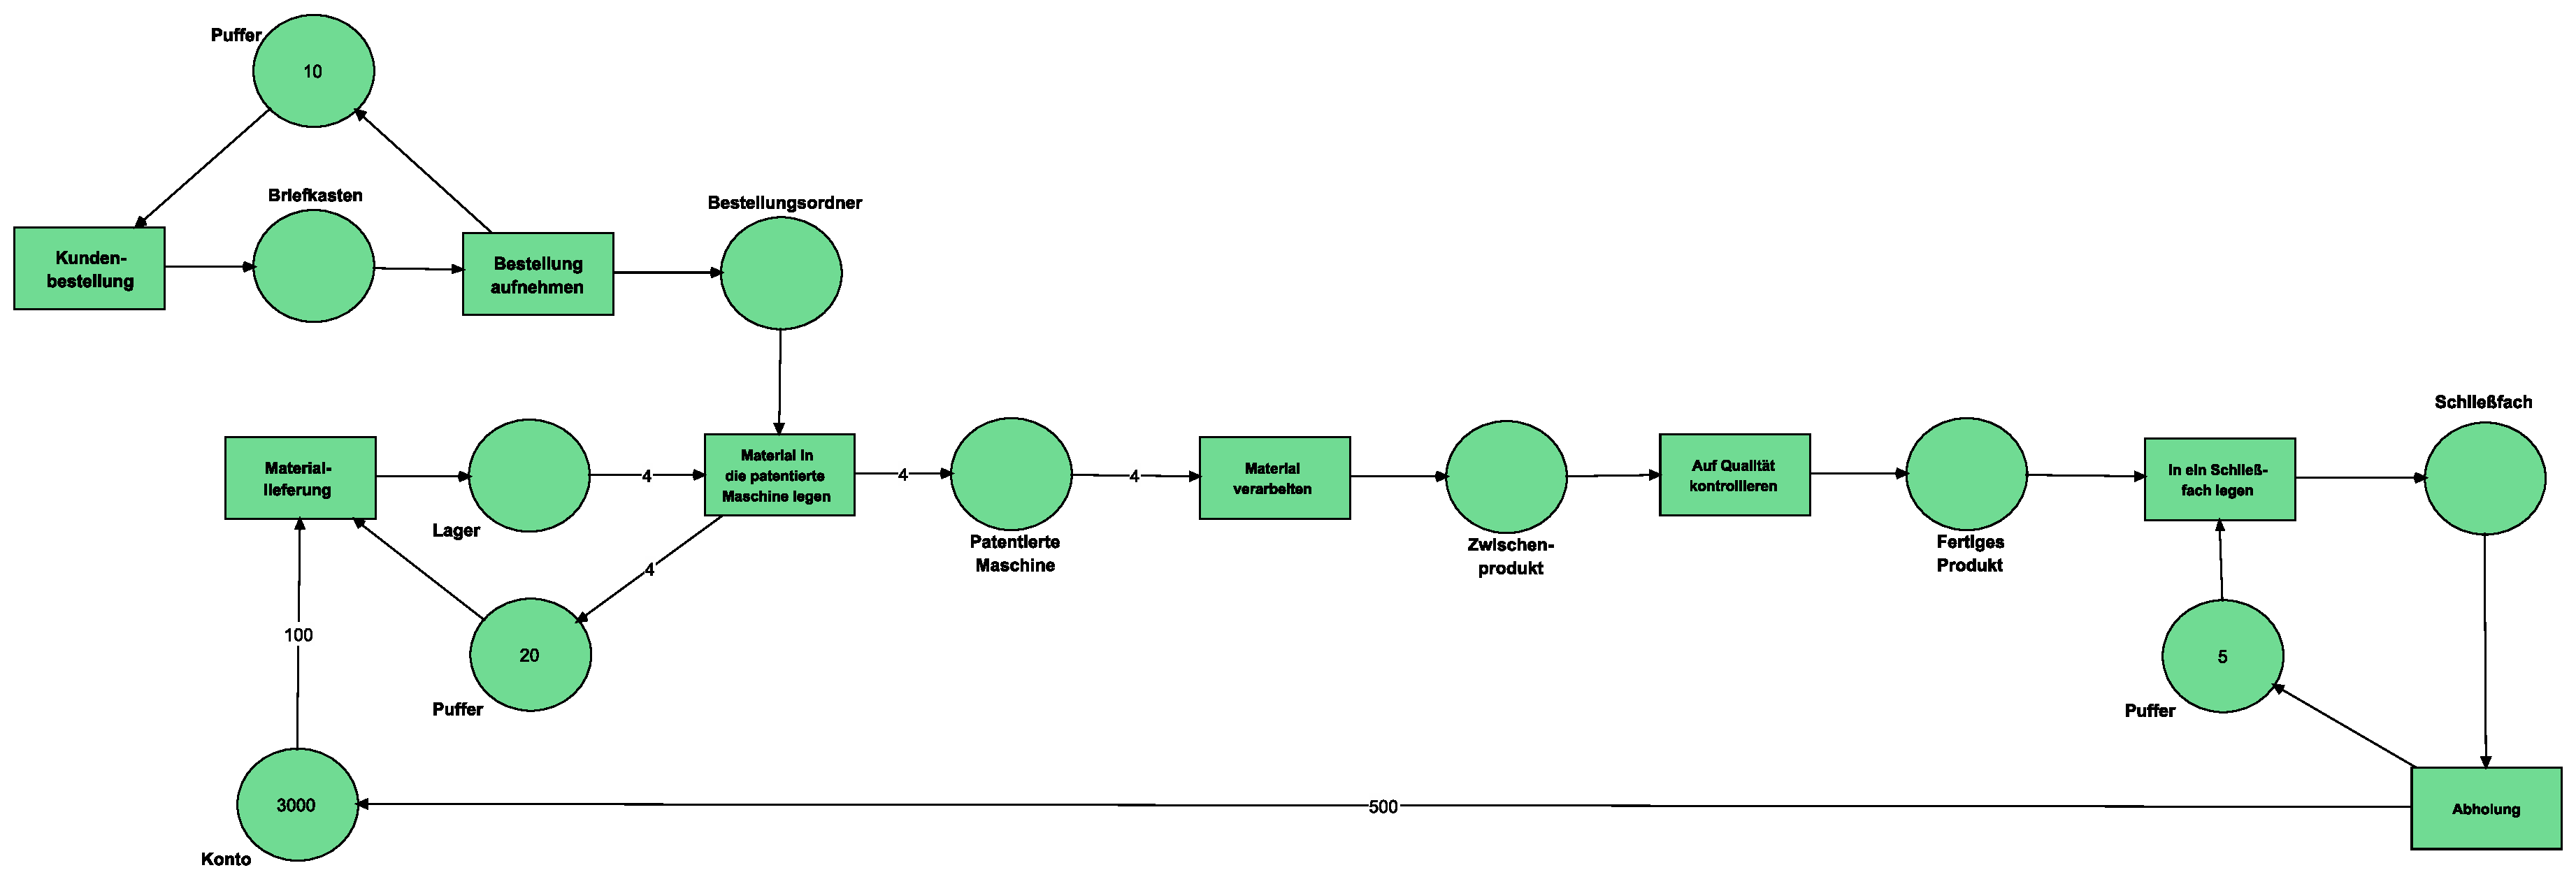
\includegraphics[scale=0.28,trim={0mm 0mm 0mm 0mm},clip]{Aufgabe_7-5/Aufgabe_7-5-6.pdf}
}\\
In diesem P/T-Netz gibt es drei Puffer, die die Größe von Briefkasten, Lager und Schließfach begrenzen. Außerdem wurde ein Konto hinzugefügt, um die Gutschriften zu organisieren. Die vorgegebenen Werte für das Konto und dessen Kanten sind dabei nur nach dem Kriterium gewählt, dass das Netz lebendig bleibt. Das Problem mit der Qualitätskontrolle ist nicht mit P/T-Netzen lösbar, da es keine Fallunterscheidung gibt.
\subsection{}

Ein Problem ist das in unserem P/T-Netz die Kapazitäten und Geldwerte nur Dummys sind. Die Kundenfirma kann hier Abhilfe schaffen indem sie Zahlen liefert. Anschließend prüfen wir erneut ob die Modulierte Produktion weiterhin ohne Probleme abläuft.

Das Abholschließfach ist für alle Kunden zugänglich unabhängig davon ob eine Bestellung für den jeweiligen Kunden darin enthalten ist. Das mag bei einem kleinen Betrieb mit wenigen Kunden funktionieren, ist mit wachsender Unternehmensgröße und Kundenzahl aber Sicherheitslücke durch die es zu Verlusten für die Firma kommen kann, zum Beispiel durch Diebstahl. Hier sollten die Firmengründer noch einmal überlegen ob sie nicht lieber einzelne Abholplätze für die Kunden haben.

Auch der in unserem Modell dargestellte Austausch von Endprodukt gegen Geld bei Abholung der Ware ist nicht gewährleistet wenn es sich um ein offenes Schließfach handelt.

\end{document}